\chapter{Diseño de la experimentación}\label{cap:disegno_experimento}

La experimentación se lleva a cabo ejecutando los 3 problemas explicados en los capítulos anteriores, considerando tres etapas distintas. La tabla \ref{tab:diseno_experimental} presenta de manera esquemática el diseño experimental completo. La primera columna de la tabla representa cada uno de los problemas y la primera fila corresponde a las distintas etapas de la experimentación realizada. En la segunda columna se encuentran los algoritmos redescubiertos, basados en sus componentes elementales para los problemas básicos que se encuentran en la literatura mediante la PG. La tercera columna, que corresponde a la versión generalizada, presenta los algoritmos generados mediante la PG utilizando los componentes elementales que permitieron redescubrir los algoritmos de la primera columna. Finalmente, la cuarta columna corresponde a algoritmos que son encontrados mediante la PG, considerando los componentes elementales y de mejora o constructivos que permiten refinar los resultados.

\begin{table}[H]
	\centering
	\caption{Resumen del diseño experimental.}
	\begin{tabular}{llll}
				& Etapa I		& Etapa II						& Etapa III\\\hline
		PCMR	& $A_{11}(g_1)$	& $A_{12}(g_1, g_2, g_3)$		& $A_{13}(g_1, g_2, g_3)$\\
		PACMG	& $A_{21}(g_1)$	& $A_{22}(g_1, g_2, g_3, g_4)$	& $A_{23}(g_1, g_2, g_3, g_4)$\\
		PVVG	&				& $A_{32}(g_1, g_2)$			& $A_{33}(g_1, g_2)$\\\hline
	\end{tabular}
	\label{tab:diseno_experimental}
\end{table}

La estrategia seguida para obtener los algoritmos que se presentan en la tabla \ref{tab:diseno_experimental}, considera la incorporación gradual de nuevos terminales que permiten encontrar mejores resultados computacionales para cada uno de los problemas estudiados. En el caso de los algoritmos de la \textit{Etapa I}, se utilizan los componentes elementales del algoritmo de Prim y Dijkstra, además de componentes adicionales que permiten dar diversidad a la evolución los cuales son utilizados como terminales en la GAA. Los algoritmos de la \textit{Etapa II} utilizan los mismos terminales que en el caso de la \textit{Etapa I}, pero adaptados a las características propias de cada problema en particular. Para los algoritmos de la \textit{Etapa III}, son utilizados los mismos terminales de la \textit{Etapa II}, además de terminales de mejora que  permiten refinar los resultados obtenidos. Por ejemplo, el término $A_{23}(g1, g2, g3, g4)$ corresponde a un algoritmo que es encontrado para el problema 2 (PACMG) en el experimento 3 (versión generalizada con terminales de refinamiento), considerando los grupos de instancias $g1$, $g2$, $g3$ y $g4$.


%DESCOMENTAR ESTAS LÍNEAS SI EL CAPÍTULO TIENE FIGURAS O TABLAS
\addtocontents{lof}{{\bf \noindent Figuras del capítulo \arabic{chapter}}}
\addtocontents{lot}{{\bf \noindent Tablas del capítulo \arabic{chapter}}}

\section{Lógica del diseño}\label{cap:logica_diseno}

Para realizar la evaluación propuesta se desarrollan ocho experimentos generando algoritmos utilizando la PG, de los cuales dos corresponden a redescubrir los algoritmos polininomiales Dikjstra correspondientes al PCM  y Prim, que da solución al PACCM utilizando sus componentes elementales como terminales. Posteriormente tres experimentos que consisten en utilizar los componentes elementales del algoritmo Dijkstra para el PCMR y  Prim para el PACMG y PVVG. Finalmente, tres experimentos que utilicen componentes elementales de los algoritmos polinomiales, más algunas componentes de refinamiento que permiten mejorar los resultados. Los experimentos relacionados a la PG siguen la estructura utilizada por otros autores para la GAA \citep{contreras_2013, drake_2014,parada_2015}. Los experimentos son los siguientes:

\begin{itemize}
  \item \textbf{Experimento 1}: tiene por objetivo realizar la GAA utilizando la PG para redescubrir el algoritmo Dijkstra.
  \item \textbf{Experimento 2}: tiene por objetivo realizar la GAA utilizando la PG para redescubrir el algoritmo Prim.
  \item \textbf{Experimento 3}: tiene por objetivo realizar la GAA utilizando la PG implementando los componentes elementales del algoritmo de Dijkstra, los cuales se adaptan para el PCMR.
  \item \textbf{Experimento 4}: tiene por objetivo realizar la GAA utilizando la PG implementando componentes elementales del algoritmo de Prim, los cuales se adaptan para el PACMG.
  \item \textbf{Experimento 5}: tiene por objetivo realizar la GAA utilizando la PG implementando componentes elementales del algoritmo de Prim, los cuales se adaptan para el PVVG.
  \item \textbf{Experimento 6}: tiene por objetivo realizar la GAA utilizando la PG ocupando los mismos componentes que en el experimento 3 y componentes de mejora para el PCMR.
  \item \textbf{Experimento 7}: tiene por objetivo realizar la GAA utilizando la PG ocupando los mismos componentes que en el experimento 4 y componentes de mejora para el PACMG.
  \item \textbf{Experimento 8}: tiene por objetivo realizar la GAA utilizando la PG ocupando los mismos componentes que en el experimento 5 y componentes de mejora para el PVVG.

\end{itemize}

\section{Metodología del experimento}
\label{cap:experimento_tradicional}

Para el desarrollo de este experimento se utiliza la PG tradicional que fue descrita en la sección \ref{cap:pg}. Este experimento está dividido en dos etapas: proceso de evolución y el proceso de evaluación.

\subsection{El proceso evolutivo}

Se considera un proceso de aprendizaje para identificar la combinación adecuada de componentes que permitan resolver el problema. Para realizar el proceso evolutivo, son necesarios los siguientes pasos:

\begin{itemize}
  \item Definir una estructura de datos acorde al problema.
  \item Definir un conjunto de funciones y terminales que cumplan con las propiedades de suficiencia y clausura.
  \item Construir una función de evaluación acorde al problema para evaluar el rendimiento de los algoritmos generados.
  \item Seleccionar un conjunto de instancias del problema para adaptar los algoritmos a generar.
  \item Determinar los métodos de evolución y el valor de los parámetros de control del proceso evolutivo.
  \item Ejecutar el proceso evolutivo un número determinado de veces y recopilar estadísticas de los individuos generados.
  \item Seleccionar un conjunto de individuos para ser estudiados.
\end{itemize}

\subsection{El proceso de evaluación}

El proceso de evaluación mide el desempeño computacional que poseen los algoritmos generados en el proceso evolutivo. El desempeño de los algoritmos se determina a partir de que tan efectivos son para resolver el problema y cuánto tiempo tardan en hacerlo. Para esto se selecciona un conjunto de instancias distinto al grupo utilizado en la evolución. Los algoritmos son evaluados en este nuevo conjunto y para medir su calidad se utiliza el error relativo promedio(ERP), que consiste en el error relativo de los algoritmos obtenidos. Para cada grupo de instancias de evaluación $S$, se determina el porcentaje promedio por el cual el beneficio obtenido $z_{i}$ se encuentra distanciado de la mejor solución $o_{i}$ para cada instancia del conjunto $S$. Esto se representa en la ecuación \ref{eq:ERP_cap3}, donde $n_{s}$ representa el número de instancias del conjunto $S$.

\begin{equation}
  \label{eq:ERP_cap3}
  ERP_{s} =  \frac{1}{n_{s}} \cdot \sum\limits_{i=1}^{n_{s}} \frac{z_{i} - o_{i}}{z_{i}} \cdot 100\%
\end{equation}


\section{Consideraciones generales}
\label{cap:consideraciones}

Para trabajar con la PG en los ocho experimentos, se tienen en consideración algunos aspectos comunes tales como: el diseño, construcción, parametrización, calibración y \textit{testing} que se realizan previo a la ejecución de la PG. Esto debido a que es un proceso iterativo en cada experimento, y los efectos de un cambio en el diseño deben implementarse junto con realizar \textit{testing} para conocer sus efectos reales. 

Se realiza a continuación una descripción de las consideraciones.

\subsection{Resultados}

En los experimentos se busca encontrar algoritmos que solucionen los problemas planteados en la hipótesis, adicionalmente, estos resultados deben dar resultados similares o mejores a los obtenidos en trabajos previos.

\subsection{Instancias}

En los experimentos se utilizan instancias disponibles en la \textit{web} para uso investigativo y reconocidas por la comunidad científica asociada al área, las cuales difieren en cantidad para cada problema.
%La complejidad, división y cantidad a utilizar es especificada en el capítulo correspondiente al diseño del experimento de cada problema.

\subsection{Ejecuciones}

Aunque la PG utiliza generación aleatoria de números, es decir, una semilla distinta para cada ejecución, se observa que bastan tres ejecuciones para probar que los resultados son estadísticamente verdaderos. Según \cite{cantu_2003, li_2004} no es necesario realizar múltiples ejecuciones, ya que esto está sujeto a varios factores, como la variabilidad de las funciones, terminales, el problema en sí,  entre otros. Es por esto que se realizó un \textit{test} estadístico, utilizando la herramienta STATA (\textit{Data analysis and statistical software}) para comprobar si los datos se encuentran normalizados, para luego analizar si existe diferencia entre los resultados entregados por cada una de las ejecuciones realizadas. 
%En la Figura xx se puede ver los resultados de tres ejecuciones de la PG, donde el mejor individuo de cada una de ellas es evaluado en las 10 instancias con que se realizó la evolución. El \textit{test} de \textit{Shapiro-Wilk} da como resultado que los valores se encuentran normalizados o en algunos casos no existe observación (los resultados son iguales). Posteriormente, se realizó un \textit{test} de ANOVA que con 95\% de confiabilidad intenta probar si los valores poseen alguna diferencia significativa, resultando que no es posible determinar que exista esta diferencia.

%\begingroup
%    \centering
%    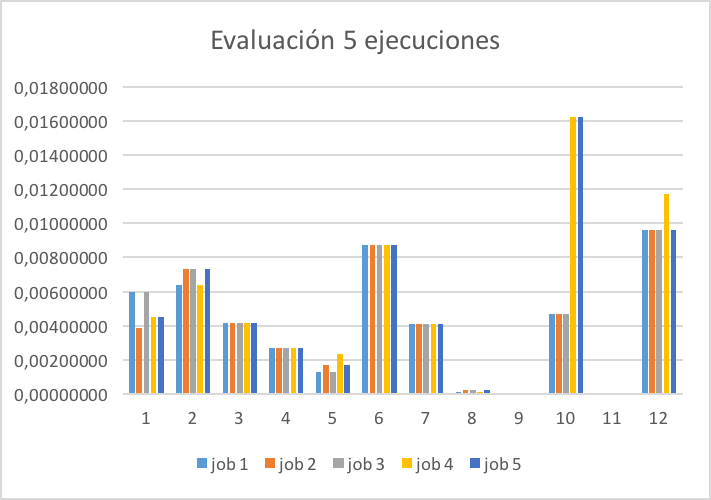
\includegraphics[width=14cm]{images/cap3/ejecuciones.png}
%    \captionof{figure}{Evaluación del mejor individuo sobre el conjunto de adaptación (Elaboración propia, 2015)}\label{fig:ejecuciones}
%\endgroup


\section{Estructuras de datos de los problemas}

Los algoritmos generados fueron construidos utilizando varias estructuras de datos. Las estructuras se diseñaron a partir de las caracteristicas de cada problemática y sus terminales y funciones. A continuación se dan a conocer los componentes de la estructura de datos para cada uno de los problemas:
 
%\paragraph{Algoritmo de Prim}
%\paragraph{Algoritmo de Dijkstra}

\paragraph{PCMR}

\begin{itemize}

\item \emph{Listas de Adyacencia de Grafo unidireccional (LAGU)}: Se guarda en esta lista de adyacencia, el grafo correspondiente a las instancias de evolución de los algoritmos. Este dato es estático, pues solo corresponde a información que deben leer los individuos y resolver durante la evolución.

\item \emph{Listas de incidencia de Grafo unidireccional (LIGU)}: Se guarda en esta lista de incidencia, el grafo correspondiente a las instancias que es usada en la evolución de los algoritmos, donde se busca almacenar las aristas que llegan a los nodos. Este dato es estático, pues solo corresponde a información que deben tomar los individuos y resolver durante la evolución.

\item \emph{Lista de etiquetas de solución (LES)}: Lista con las etiquetas del grafo. Se tiene una lista de etiquetas de tamaño $DIM_i$, siendo $i$ la instancia correspondiente de la etiqueta. Esta se inicializa con los valores de recursos y costo en infinito y con antecesor nulo.

\item \emph{Lista de nodos sin revisar (LNSR)}: Posee todos los nodos que no han sido etiquetados, vale decir, no se ha cambiado en la estructura \emph{LES}.

\item \emph{Último (U)}: Es el último nodo marcado que fue de menor costo y que, a partir de él, se siguen etiquetando nodos.

%\item \emph{Booleano de verificación de cambios } (HC): Toma el valor de verdadero cuando se realiza un cambio en \emph{LE} o en \emph{U}, y falso cuando no se ha hecho ningún cambio.
\end{itemize}

\paragraph{PACMG}

\begin{itemize}
\item Matriz de adyacencia (MAAC): En esta estructura se almacenan las distancias entre nodos, considerando la distancia euclidiana estipulado en las instancias. Las dimensiones de esta matriz son de $n x n$, dónde $n$ es la cantidad de nodos.

\item Mapa de relación cluster-nodo (MACN): Esta estructura almacena la relación existente entre el cluster y las características del nodo, además de almacenar por cada nodo, todos los posibles nodos con los que se puede conectar.

\item Listas de listas de la solución (LLS): En esta estructura se almacena el árbol de solución, donde cada posición i de la lista (raiz), contiene los nodos asociados $i$ (hijos).

\item Lista de Solución (LSAC): Almacena una lista de enteros, siendo estos, los nodos incluidos en la solución por cada cluster.

\end{itemize}	
	
\paragraph{PVVG}

\begin{itemize}
\item Matriz de adyacencia (MAVV): En esta estructura se almacenan las distancias entre nodos, considerando la distancia euclidiana estipulado en las instancias. Las dimensiones de esta matriz son de $N x N$, dónde $N$ es la cantidad de nodos (Referencia Parada Teoría de grafos).
  
\item Lista de nodos (LN): En esta estructura se almacenan estructura de nodos. Dicha estructura posee las características primordiales de un nodo: id, coordenadas y clúster al cual pertenece el nodo.  

\item Listas de adyacencia de clúster (LAC): Es una lista de listas. Cada posición i de la lista, contiene una lista de nodos asociados al clúster $i+1$ (Referencia Montgomery diseño y análisis).
 
\item Lista de nodos cercanos al centro (LNCC): Se construye una lista de nodos ordenados de menor a mayor según el centro de la instancia. El tamaño de esta estructura solo almacena $n/2$ nodos.
 
\item Lista de nodos cercanos al centro (LNLC):  Se construye una lista de nodos ordenados de menor a mayor según el centro de la instancia. El tamaño de esta estructura solo almacena $n/2$ nodos.

\item Lista de Solucion (LSVV): Almacena una lista de enteros, siendo estos, los nodos incluidos en la solución. El circuito se cierra conectado conectando el último de nodo de la lista con el primero de esta esta estructura. 
 
\end{itemize}	
	
\section{Identificación de Componentes Elementales}\label{cap:identificacion_componentes}

En esta sección se presenta el análisis para la obtención de los componentes elementales de los problemas fáciles.

\subsection{Descomponiendo Algoritmo Dijkstra}
El algoritmo de Dijkstra permite resolver de forma polinomial el PCM y en el algoritmo \ref{alg:alg41} se presenta su pseudocódigo.


\begin{algorithm}[H]
    \begin{algorithmic}[1]
        \STATE {\em Inicializar Etiquetas con antecesor nulo y costo INFINITO}
        \STATE {\em Inicializar una lista L con Todos los vétices del Grafo}
        \STATE {\em Etiquetar Vértice Inicial=[-,0]}
        \STATE {\em Marcar X = vértice Inicial}
        \STATE {\em Eliminar Vértice Incial de L}
        \WHILE {{\em Quedan Vértices en lista L}}
            \STATE {\em Actualizar etiquetas vecinos de X solo si el costo es menor.}
            \STATE {\em Buscar en L, el nodo con Etiqueta con costo más bajo (Nmin).}
            \STATE {\em Macar X=Nmin.}
            \STATE {\em Eliminar Nmin de L}
        \ENDWHILE
    \end{algorithmic}
    \caption{Algoritmo de Dijkstra}\label{alg:alg41}
\end{algorithm}

En el algoritmo \ref{alg:alg41}, de la línea 1 hasta la 5 se inicializan las estructuras de datos, mientras que en la línea 6 se puede observar el ciclo que permite realizar las iteraciones hasta encontrar el camino mínimo. La línea 7 es la encargada de actualizar las etiquetas de los vecinos del vértice seleccionado, la línea 8 busca en la lista de nodos disponibles el vértice seleccionado, la línea 9 es la encargada de marcar el vértice en la solución y la línea 10 es la que elimina el vértice marcado de la lista de vértices disponibles.

De esta forma el algoritmo se ejecuta hasta que todos los vértices hayan sido marcados. Esto se cumple con el criterio de término del ciclo \emph{while} del pseudocódigo, ya que a medida que se extraen los nodos de la lista \emph{L}, se van marcando y etiquetando los vértices del grafo.

Se puede observar que los componentes elementales del algoritmo están en la línea 6, que es la que permite que el ciclo siga hasta encontrar la solución, línea 7, encargada de actualizar las etiquetas y la línea 9  marcar el vértice en la solución. Generando así las siguientes funciones elementales:

\begin{itemize}


\item \textbf{Marca costo menor}: marca el vértice de costo menor en la solución.

\item \textbf{Etiquetar Dijkstra}: Actualiza las etiquetas del problema.

\item \textbf{Quedan vertices}: Verifica si ya se encontró el vértice final.
\end{itemize}

%Además se agregan funciones que permiten la diversidad en la evolución. Estas funciones son:


%\begin{itemize}

%\item \textbf{Etiquetador}: Cambia las etiquetas de los vecinos del último vértice marcado. Los vecinos deben ser vértices que no han sido marcados.


%\item \textbf{MarcaCostoMayor}: Elimina un vértice a la lista de vértices no marcados y es agregado como último vértice marcado. El vértice seleccionado es aquel que posea la etiqueta con mayor costo acumulado.

%\item \textbf{MarcarGradoMenor}: Elimina un vértice a la lista de vértices no marcados y es agregado como último vértice marcado. El vértice seleccionado es aquel que posea el menor grado.

%\item \textbf{MarcarGradoMayor}: Elimina un vértice a la lista de vértices no marcados y es agregado como último vértice marcado. El vértice seleccionado es aquel que posea el mayor grado.



%\item \textbf{EtiquetarVerificaPeso}: Cambia las etiquetas de los vecinos a partir del último vértice marcado verificando que el peso acumulado de la etiqueta no supere el peso máximo permitido. Si un vértice vecino ya fue etiquetado, se deja el que tenga menor costo acumulado. Si un vértice fue marcado anteriormente, no puede volver a ser etiquetado.

%\item \textbf{MarcarPonderado}: Elimina un vértice a la lista de vértices no marcados y es agregado como último vértice marcado. El vértice seleccionado es aquel que posea el menor valor que resulte de la multiplicación entre su peso acumulado y su costo acumulado.

%\item \textbf{MejorarDijkstra}: Cambia la etiqueta del último vértice marcado a partir de los vértice incidentes en él. Se realiza el cambio si el costo acumulado de la nueva etiqueta es menor al que va a reemplazar.

%\item \textbf{MejorarDijkstraPeso}: Cambia la etiqueta del último vértice marcado a partir de los vértice incidentes en él verificando que el peso acumulado de la etiqueta no supere el peso máximo permitido. Se realiza el cambio si el costo acumulado de la nueva etiqueta es menor al que va a reemplazar.

%\end{itemize}

%\item \textbf{MarcaPesoMenor}: Elimina un vértice a la lista de vértices no marcados y es agregado como último vértice marcado. El vértice seleccionado es aquel que posea la etiqueta con menor peso cumulado.

\subsection{Descomponiendo Algoritmo Prim}
El algoritmo de Prim permite resolver de forma polinomial el problema del aŕbol de cobertura de costo mínimo y en el algoritmo \ref{alg:alg42} se presenta su pseudocódigo.

%\subsection{Descomponiendo Algoritmo Prim}
\begin{algorithm}[H]
    \caption{Algoritmo de Prim}\label{alg:alg42}
    \begin{algorithmic}[1]
    	\STATE Inicializar una lista L con Todos los vétices del árbol
        \STATE Inicializar el árbol con un vértice arbitrario.
        \WHILE {\em Quedan Vértices sin utilizar}
        \STATE Añadir la arista de menor peso que se conecte con el árbol.
        \STATE Eliminar la arista de menor peso de la lista L.
        \ENDWHILE
    \end{algorithmic}
\end{algorithm}

En el algoritmo \ref{alg:alg42}, en las líneas 1 y 2 se inicializan las estructuras de datos que almacena el árbol de solución, mientras que en la línea 3 se puede observar el ciclo que permite realizar las iteraciones hasta encontrar el aŕbol de cobertura de costo mínimo, la línea 4 es la que va agregando cada vértice al árbol, y finalmente la línea 5 elimina el vértice agregado al árbol. De esta forma el algoritmo se ejecuta hasta que todos los vértices hayan sido agregados al árbol.

Se puede observar que los componentes elementales del algoritmo están en la línea 3, que es la que permite que el ciclo siga hasta encontrar la solución y la línea 4, que permite ir construendo el árbol agregando la arísta de costo menor. Generando así los siguientes funciones elementales para el redescubrimiento:

\begin{itemize}

\item \textbf{Quedan Cluster}: Verifica si aún existen vértices disponibles que no sean parte de la solución.

\item \textbf{IniAristaMenorMasNodos}: Agrega dos vértices iniciales a la solución parcial, los cuales son parte de la arista de menor costo.

\item \textbf{constAristaMenor}: Agrega un nuevo vértice a la solución parcial. El vértice seleccionado es aquel que tiene la arista de menor costo entre los nodos que pertenecen a la solución.
\end{itemize}

%Además se agregan terminales que permiten la diversidad en la evolución. Estas funciones son:


%\begin{itemize}
%
%\item \textbf{IniAristaMenor}: Agrega dos vértices iniciales a la solución parcial, los cuales son parte de la arista de menor costo.

%\item \textbf{IniAristaMayor}: Agrega dos vértices iniciales a la solución parcial, los cuales son parte de la arista de mayor costo.

%\item \textbf{constAristaMayor}: Agrega un vértice a la solución parcial. El vértice seleccionado es aquel que tiene la arista de mayor costo que conecte a un clúster que no se encuentre en la solución

%\item \textbf{constKruskalMenor}: Agrega dos vértices que no pertenecen a la solución parcial. Los vértices forman parte de la arista de menor costo encontrada entre los clusters que no se encuentre en la solución.

%\item \textbf{constKruskalMayor}: Agrega dos nuevos vértices a la solución parcial. Los vértices forman parte de la arista de mayor costo encontrada entre los clusters que no forman parte de la solución.

%\end{itemize}

\section{Definición de funciones y terminales}\label{cap:definicion_terminales}

Se define como funciones todos aquellos componentes que requieren de argumentos y, como terminales, todos aquellos componentes que no lo requieran, donde además, tanto funciones como terminales deben retornar algún valor \citep{koza1992genetic}. 

Las funciones y terminales son las operaciones elementales de las estructuras de datos anteriormente definidas. Por lo tanto, su definición es fundamental para generar algoritmos con la capacidad de utilizar dichas estructuras con el fin de alcanzar una solución que minimice el costo para el PCMR, PACMG y PVVG. Se construyen terminales en base a los componentes elementales de los problemas fáciles, además de algunos terminales de refinamiento, y funciones que permitan operar en diversas combinaciones sobre estos terminales.

%Los elementos del conjunto de funciones y terminales deben cumplir con las propiedades de suficiencia y clausura \citep{poli_2008}. Las funciones y terminales cumplen la propiedad de clausura, ya que todas retornan un valor verdadero o falso, y las funciones solo pueden recibir parámetros de entrada de ese tipo. La propiedad de suficiencia se cumple con cada uno de los terminales, ya que éstos se encargan de agregar o eliminar vértices a las soluciones.


\subsection{Conjunto de funciones}

Las funciones que conforman los algoritmos generados para los ocho experimentos contienen instrucciones básicas utilizadas en su mayoría por todos los lenguajes de programación. Desde el punto de vista de la PG, las funciones corresponden a los nodos internos del árbol \citep{koza_poli_2005} y estas se presentan a continuación:

\begin{itemize}

\item \emph{While(a1,a2):} Realiza el argumento \emph{a2} mientras el argumento \emph{a1} retorne verdadero. Lo característico de este \emph{While} es tiene como límite de iteraciones el número total de elementos. Esta condición son necesaria debido a que el argumento \emph{a1} del \emph{While} puede retornar siempre verdadero, rompiendo así la propiedad de clausura de la evolución (Koza et al., 2003). La función retorna verdadero si al menos realiza un cambio en el total de iteraciones realizadas. Si en ninguna de las iteraciones ejecutadas realiza un cambio en la estructura de datos de solución, retorna falso.

\item \emph{If\_then(a1,a2):} Se ejecuta el argumento \emph{a1}. Si éste retorna verdadero, se ejecuta el argumento \emph{a2} y la función retorna verdadero. En caso contrario, no se ejecuta \emph{a2} y la función retorna falso.

\item \emph{And(a1,a2):} Se ejecuta el argumento \emph{a1} y el argumento \emph{a2}. La función retorna verdadero si \emph{a1} y \emph{a2} son verdaderos, en cualquier otro caso retorna falso.

\item \emph{Or(a1,a2):} Se ejecuta el argumento \emph{a1} y el argumento \emph{a2}. La función retorna falso si \emph{a1} y \emph{a2} son falsos, en cualquier otro caso retorna verdadero.

\item \emph{Not(a1):} Se ejecuta el argumento \emph{a1}. La función retorna la negación lógica del resultado del argumento.

\item \emph{Equal(a1,a2):} Se ejecuta el argumento \emph{a1} y se ejecuta el argumento \emph{a2}. Si el argumento \emph{a1} retorna lo mismo que el argumento \emph{a2}, la función retorna verdadero, en caso contrario, retorna falso.
\end{itemize}

\subsection{Conjunto de terminales}

Los terminales son funciones diseñadas para cada uno de los problemas. De acuerdo a la definición de la PG, un terminal es un nodo hoja \citep{koza_poli_2005}. Cada uno de los terminales es una heurística elemental capaz de modificar la estructura de datos definida generando nuevas soluciones. Los terminales a utilizar son:

\subsubsection*{Redescubrimiento de Dijkstra}

\begin{itemize}

\item \textit{MarcaCostoMenor}: Elimina un vértice de la lista de vértices no marcados y es agregado como último vértice marcado. El vértice seleccionado es aquel que posea la etiqueta con menor costo acumulado. Retorna verdadero si se logra marcar un vértice, falso en el caso contrario.

\item \textit{EtiquetarDijkstra}: Cambia las etiquetas de los vecinos a partir del último vértice marcado. Si un vértice vecino ya fue etiquetado, se selecciona la etiqueta que posea el menor costo acumulado. Si un vértice fue marcado anteriormente, no puede volver a ser etiquetado. Retorna verdadero si se logra etiquetar un vértice, falso en el caso contrario.

\item \textit{QuedanVertices}: Verifica si aún existen vértices que no han sido marcados. Retorna verdadero si quedan vértices por recorrer, falso en el caso contrario.

\item \textit{Etiquetador}: Cambia las etiquetas de los vecinos del último vértice marcado. Los vecinos deben ser vértices que no han sido marcados. Retorna verdadero si se logra cambiar las etiquetas de los vecinos, falso en el caso contrario.

\item \textit{MarcaCostoMayor}: Elimina un vértice a la lista de vértices no marcados y es agregado como último vértice marcado. El vértice seleccionado es aquel que posea la etiqueta con mayor costo acumulado. Retorna verdadero si se logra marcar un vértice, falso en el caso contrario.

\item \textit{MarcarGradoMenor}: Elimina un vértice a la lista de vértices no marcados y es agregado como último vértice marcado. El vértice seleccionado es aquel que posea el menor grado. Retorna verdadero si se logra marcar un vértice, falso en el caso contrario.

\item \textit{MarcarGradoMayor}: Elimina un vértice a la lista de vértices no marcados y es agregado como último vértice marcado. El vértice seleccionado es aquel que posea el mayor grado. Retorna verdadero si se logra marcar un vértice, falso en el caso contrario.

\end{itemize}

\subsubsection*{Redescubrimiento de Prim}

\begin{itemize}

\item \textit{QuedanCluster}: Verifica si aún existen vértices disponibles que no sean parte de la solución. Retorna verdadero si aún quedan clúster por seleccionar, falso en el caso contrario.

%\item \textbf{IniAristaMenorMasNodos}: Agrega dos vértices iniciales a la solución parcial, los cuales son parte de la arista de menor costo.

\item \textit{constAristaMenor}: Agrega un nuevo vértice a la solución parcial. El vértice seleccionado es aquel que tiene la arista de menor costo entre los nodos que pertenecen a la solución. Retorna verdadero si se logra agregar el  vértice a la solución, falso en el caso contrario.

\item \textit{IniAristaMenor}: Agrega dos vértices iniciales a la solución parcial, los cuales son parte de la arista de menor costo. Retorna verdadero si se logra agregar los dos vértices a la solución, falso en el caso contrario.

\item \textit{IniAristaMayor}: Agrega dos vértices iniciales a la solución parcial, los cuales son parte de la arista de mayor costo. Retorna verdadero si se logra agregar los dos vértices a la solución, falso en el caso contrario.

\item \textit{constAristaMayor}: Agrega un vértice a la solución parcial. El vértice seleccionado es aquel que tiene la arista de mayor costo que conecte a un clúster que no se encuentre en la solución. Retorna verdadero si se logra agregar el  vértice a la solución, falso en el caso contrario.

\item \textit{constKruskalMenor}: Agrega dos vértices que no pertenecen a la solución parcial. Los vértices forman parte de la arista de menor costo encontrada entre los clusters que no se encuentre en la solución. Retorna verdadero si se logra agregar los dos vértices a la solución, falso en el caso contrario.

\item \textit{constKruskalMayor}: Agrega dos nuevos vértices a la solución parcial. Los vértices forman parte de la arista de mayor costo encontrada entre los clusters que no forman parte de la solución. Retorna verdadero si se logra agregar los dos vértices a la solución, falso en el caso contrario.

\end{itemize}

\subsubsection*{PCMR}

Para el experimento 3 se utilizan los mismos terminales que para el redescubrimiento del Djkstra, pero acorde a las restricciónes, características y estuctura del PCMR:

\begin{itemize}

\item \textit{MarcaCostoMenor}: Elimina un vértice a la lista de vértices no marcados y es agregado como último vértice marcado. El vértice seleccionado es aquel que posea la etiqueta con menor costo acumulado.

\item \textit{MarcaPesoMenor}: Elimina un vértice a la lista de vértices no marcados y es agregado como último vértice marcado. El vértice seleccionado es aquel que posea la etiqueta con menor peso cumulado. 

\item \textit{MarcarGradoMenor}: Elimina un vértice a la lista de vértices no marcados y es agregado como último vértice marcado. El vértice seleccionado es aquel que posea el menor grado.

\item \textit{MarcarGradoMayor}: Elimina un vértice a la lista de vértices no marcados y es agregado como último vértice marcado. El vértice seleccionado es aquel que posea el mayor grado.

\item \textit{MarcarPonderado}: Elimina un vértice a la lista de vértices no marcados y es agregado como último vértice marcado. El vértice seleccionado es aquel que posea el menor valor que resulte de la multiplicación entre su peso acumulado y su costo acumulado. 

\item \textit{Etiquetador}: Cambia las etiquetas de los vecinos del último vértice marcado. Los vecinos deben ser vértices que no han sido marcados.

\item \textit{EtiquetarDijkstra}: Cambia las etiquetas de los vecinos a partir del último vértice marcado. Si un vértice vecino ya fue etiquetado, se selecciona la etiqueta que posea el menor costo acumulado. Si un vértice fue marcado anteriormente, no puede volver a ser etiquetado.

\item \textit{EtiquetarVerificaPeso}: Cambia las etiquetas de los vecinos a partir del último vértice marcado verificando que el peso acumulado de la etiqueta no supere el peso máximo permitido. Si un vértice vecino ya fue etiquetado, se deja el que tenga menor costo acumulado. Si un vértice fue marcado anteriormente, no puede volver a ser etiquetado.

\end{itemize}

Para el experimento 6 se utilizan los mismos terminales que para el experimento 3 y se agregan dos terminales de refinamiento:

\begin{itemize}

\item \textit{MejorarDijkstra}: Cambia la etiqueta del último vértice marcado a partir de los vértice incidentes en él. Se realiza el cambio si el costo acumulado de la nueva etiqueta es menor al que va a reemplazar.

\item \textit{MejorarDijkstraPeso}: Cambia la etiqueta del último vértice marcado a partir de los vértice incidentes en él verificando que el peso acumulado de la etiqueta no supere el peso máximo permitido. Se realiza el cambio si el costo acumulado de la nueva etiqueta es menor al que va a reemplazar.

\end{itemize}

\subsubsection*{PACMG}

Para el experimento 4 se utilizan los mismos terminales que para el redescubrimiento de Prim, pero acorde a las restricciónes, características y estuctura del PACMG:

\begin{itemize}

\item \textit{QuedanCluster}: Verifica si aún existen vértices disponibles que no sean parte de la solución. Retorna verdadero si aún quedan clúster por seleccionar, falso en el caso contrario.

%\item \textbf{IniAristaMenorMasNodos}: Agrega dos vértices iniciales a la solución parcial, los cuales son parte de la arista de menor costo.

\item \textit{constAristaMenor}: Agrega un nuevo vértice a la solución parcial. El vértice seleccionado es aquel que tiene la arista de menor costo entre los nodos que pertenecen a la solución. Retorna verdadero si se logra agregar el  vértice a la solución, falso en el caso contrario.

\item \textit{IniAristaMenor}: Agrega dos vértices iniciales a la solución parcial, los cuales son parte de la arista de menor costo. Retorna verdadero si se logra agregar los dos vértices a la solución, falso en el caso contrario.

\item \textit{IniAristaMayor}: Agrega dos vértices iniciales a la solución parcial, los cuales son parte de la arista de mayor costo. Retorna verdadero si se logra agregar los dos vértices a la solución, falso en el caso contrario.

\item \textit{constAristaMayor}: Agrega un vértice a la solución parcial. El vértice seleccionado es aquel que tiene la arista de mayor costo que conecte a un clúster que no se encuentre en la solución. Retorna verdadero si se logra agregar el  vértice a la solución, falso en el caso contrario.

\item \textit{constKruskalMenor}: Agrega dos vértices que no pertenecen a la solución parcial. Los vértices forman parte de la arista de menor costo encontrada entre los clusters que no se encuentre en la solución. Retorna verdadero si se logra agregar los dos vértices a la solución, falso en el caso contrario.

\item \textit{constKruskalMayor}: Agrega dos nuevos vértices a la solución parcial. Los vértices forman parte de la arista de mayor costo encontrada entre los clusters que no forman parte de la solución. Retorna verdadero si se logra agregar los dos vértices a la solución, falso en el caso contrario.

\end{itemize}

Para el experimento 7 se utilizan los mismos terminales que para el experimento 4 y se agregan cinco terminales de refinamiento:

\begin{itemize}

\item \textit{MejorarConexionAltura2}: mejora la solución actual  reestructurando un subárbol de altura 2 perteneciente a la solución mediante el uso del prim modificado. Posteriormente se conecta al vértice del que fue desconectado al comienzo. 

\item \textit{MejorarConexionAltura3}: mejora la solución actual  reestructurando un subárbol de altura 3 perteneciente a la solución mediante el uso del prim modificado. Posteriormente se conecta al vértice del que fue desconectado al comienzo.

\item \textit{MejorarConexionAltura4}: mejora la solución actual  reestructurando un subárbol de altura 4 perteneciente a la solución mediante el uso del prim modificado. Posteriormente se conecta al vértice del que fue desconectado al comienzo.

\item \textit{MejoraConexiónCluster}: Busca una mejora de la solución actual desplazando las aristas de un cluster por todos sus vértices, manteniendo el vértice que mejore la solución. Este proceso finaliza cuando se recorren todos los clúster.

\item \textit{CortarConexiónSubárbolMayorAltura}: Corta la rama con mayor altura de la solución actual. 

\end{itemize}


\subsubsection*{PVVG}

Para el experimento 5 se utiliza una adaptación de los componentes elementales del redescubrimiento de Prim, pero acorde a las restricciónes, características y estuctura del PVVG:

\begin{itemize}

\item \textit{AgregarMejorVecino}: Busca en los vertices disponibles, el vertice que agregue el menor costo al circuito y es agregado al final de éste, donde el clúster al que pertenece el vértice no forme parte de la solución parcial. Retorna verdadero si agrega el vertice, falso en caso contrario.

\item \textit{AgregarPeorVecino}: Busca en los vertices disponibles, el vertice que agregue el mayor costo al circuito y es agregado al final de éste, donde el clúster al que pertenece el vértice no forme parte de la solución parcial. Retorna verdadero si agrega la ciudad, falso en caso contrario.

\item \textit{AgregarCercaCentro}: Busca el vértice más cercano a las coordenadas del centro que se encuentre disponible. Si encuentra un vértice, éste es agregado al final del circuito, donde el clúster al que pertenece el vértice no forme parte de la solución parcial. Retorna verdadero si agrega la ciudad, falso en caso contrario.

\item \textit{AgregarLejosCentro}:	Busca el vértice más lejano a las coordenadas del centro que se encuentre disponible. Si encuentra un vértice, éste es agregado al final del circuito, donde el clúster al que pertenece el vértice no forme parte de la solución parcial. Retorna verdadero si agrega la ciudad, falso en caso contrario.

\item \textit{AgregarCercano}: Busca el vértice que al ser agregado en cualquier posición del circuito, sume el menor costo a éste. Donde el clúster al que pertenece el vértice no forme parte de la solución parcial. Por ejemplo, se tiene el circuito $[A, B, C]$ donde ingresa $D$, siendo $A->D < B->D < C->D$. El resultado luego de la inserción es $[A, D, B, C]$. Retorna verdadero si agrega la ciudad, falso en caso contrario.

\item \textit{AgregarLejano}: Busca el vértice que al ser agregado en cualquier posición del circuito, sume el mayor costo a éste. Donde el clúster al que pertenece el vértice no forme parte de la solución parcial. Por ejemplo, se tiene el circuito $[A, B, C]$ donde ingresa $D$, siendo $A->D < B->D < C->D$. El resultado luego de la inserción es $[A, B, C, D]$. Retorna verdadero si agrega la ciudad, falso en caso contrario.

\item \textit{EliminarPeorArco}: Busca en el circuito dos vertices que produzcan el peor arco (el mayor costo al circuito). Ambos vertices correspondientes al peor arco son eliminadas. Retorna verdadero si logra eliminar el arco y falso en caso contrario.

%\item AgregarArcoMenor: De forma similar a agregar cercano, busca una ciudad que al ser insertada agregue el menor costo al circuito. La diferencia está en que el menor costo es considerando el nuevo arco a formar. Por ejemplo, se tiene el circuito $[A, B, C]$ y se agrega $X$, siendo $A->X->B > B->X->C > C->X$. El resultado es $[A, X, B, C]$. Retorna verdadero si agrega la ciudad, falso en caso contrario.

%\item AgregarArcoMayor: De forma similar a agregar lejano, busca una ciudad que al ser insertada agregue el mayor costo al circuito. La diferencia en este caso se encuentra en que el mayor costo considera el nuevo arco a formar. Por ejemplo, se tiene el circuito $[A, B, C]$ y se agrega $X$, siendo $A->X->B < B->X->C < C->X$. El resultado es $[A, B, C, X]$.

\end{itemize}

Para el experimento 8 se utilizan los mismos terminales que para el experimento 5 y se agregan tres terminales de refinamiento:

\begin{itemize}

\item \textit{Invertir}: Cambia el orden de los vertices sólo en el caso en que este cambio produzca alguna mejora. El cambio se realiza mediante la inversión de las posiciones de los extremos hacia adentro. Por ejemplo, la primera se invierte con la última, la segunda con la penúltima y así sucesivamente. Retorna verdadero si logra mejorar el costo del circuito y falso en caso contrario.

\item \textit{mejoraLKH}: Optimizador que utiliza la heurística LKH. Retorna verdadero si puede realizar alguna mejora al circuito y falso en caso contrario.

\end{itemize}


%%
%terminales PVVG
%%•	Existe_cluster_en_solucion(Nodo n): Función que verifica la restricción (X.X) de la formulación matemática, es decir, si el clúster que pertenece al nodo n se encuentra dentro de la solución parcial. Retorna verdadera si el clúster al que pertenece el nodo se encuentra en la solución y falso en caso en contrario.
%%•	Agregar_a_la_solución(Nodo n):  Función que agrega al final de  LS, el nodo n. No existe retorno para esta función.
%%•	Distancia (Nodo n1, Nodo n2): Función que retorna la distancia entre nodo n1 y n2 utilizando M.
%%•	Ultimo_en_Solucion(): Retorna de LS, el último nodo insertado. Si no hay nodos insertados, Retorna el primer nodo.
%%•	Agregar_solucion_entremedio(Nodo n1, Nodo n2): Función que inserta en la solución parcial LS en la posición donde se encuentra n1, al nodo n2. En caso que no exista n1, se agrega al final.
%%•	EliminaArco(Nodo n1, Nodo n2): Elimina nodos n1 y n2 de la solución LS.
